%%%%%%%%%%%%%%%%%%%%%%%%%%%%%%%%%%%%%%%%%
% Proceedings of the National Academy of Sciences (PNAS)
% LaTeX Template
% Version 1.0 (19/5/13)
%
% This template has been downloaded from:
% http://www.LaTeXTemplates.com
%
% Original author:
% The PNAStwo class was created and is owned by PNAS:
% http://www.pnas.org/site/authors/LaTex.xhtml
% This template has been modified from the blank PNAS template to include
% examples of how to insert content and drastically change commenting. The
% structural integrity is maintained as in the original blank template.
%
% Original header:
%% PNAStmpl.tex
%% Template file to use for PNAS articles prepared in LaTeX
%% Version: Apr 14, 2008
%
%%%%%%%%%%%%%%%%%%%%%%%%%%%%%%%%%%%%%%%%%

%----------------------------------------------------------------------------------------
%	PACKAGES AND OTHER DOCUMENT CONFIGURATIONS
%----------------------------------------------------------------------------------------

%------------------------------------------------
% BASIC CLASS FILE
%------------------------------------------------

%% PNAStwo for two column articles is called by default.
%% Uncomment PNASone for single column articles. One column class
%% and style files are available upon request from pnas@nas.edu.

%\documentclass{pnasone}
\documentclass{pnastwo}

%------------------------------------------------
% POSITION OF TEXT
%------------------------------------------------

%% Changing position of text on physical page:
%% Since not all printers position
%% the printed page in the same place on the physical page,
%% you can change the position yourself here, if you need to:

% \advance\voffset -.5in % Minus dimension will raise the printed page on the 
                         %  physical page; positive dimension will lower it.

%% You may set the dimension to the size that you need.

%------------------------------------------------
% GRAPHICS STYLE FILE
%------------------------------------------------

%% Requires graphics style file (graphicx.sty), used for inserting
%% .eps/image files into LaTeX articles.
%% Note that inclusion of .eps files is for your reference only;
%% when submitting to PNAS please submit figures separately.

%% Type into the square brackets the name of the driver program 
%% that you are using. If you don't know, try dvips, which is the
%% most common PC driver, or textures for the Mac. These are the options:

% [dvips], [xdvi], [dvipdf], [dvipdfm], [dvipdfmx], [pdftex], [dvipsone],
% [dviwindo], [emtex], [dviwin], [pctexps], [pctexwin], [pctexhp], [pctex32],
% [truetex], [tcidvi], [vtex], [oztex], [textures], [xetex]

\usepackage{graphicx}
\usepackage{amsmath}
\usepackage{float}
\usepackage{todo}

%------------------------------------------------
% OPTIONAL POSTSCRIPT FONT FILES
%------------------------------------------------

%% PostScript font files: You may need to edit the PNASoneF.sty
%% or PNAStwoF.sty file to make the font names match those on your system. 
%% Alternatively, you can leave the font style file commands commented out
%% and typeset your article using the default Computer Modern 
%% fonts (recommended). If accepted, your article will be typeset
%% at PNAS using PostScript fonts.

% Choose PNASoneF for one column; PNAStwoF for two column:
%\usepackage{PNASoneF}
%\usepackage{PNAStwoF}

%------------------------------------------------
% ADDITIONAL OPTIONAL STYLE FILES
%------------------------------------------------

%% The AMS math files are commonly used to gain access to useful features
%% like extended math fonts and math commands.

\usepackage{amssymb,amsfonts,amsmath}

%------------------------------------------------
% OPTIONAL MACRO FILES
%------------------------------------------------

%% Insert self-defined macros here.
%% \newcommand definitions are recommended; \def definitions are supported

%\newcommand{\mfrac}[2]{\frac{\displaystyle #1}{\displaystyle #2}}
%\def\s{\sigma}

%------------------------------------------------
% DO NOT EDIT THIS SECTION
%------------------------------------------------

%% For PNAS Only:
\contributor{Submitted to Proceedings of the National Academy of Sciences of the United States of America}
%\url{www.pnas.org/cgi/doi/10.1073/pnas.0709640104}
\copyrightyear{2015}
\issuedate{03-16-2015}
\volume{1}
\issuenumber{1}

%----------------------------------------------------------------------------------------

\begin{document}

%----------------------------------------------------------------------------------------
%	TITLE AND AUTHORS
%----------------------------------------------------------------------------------------

\title{File Access Quorum. Secured by Multifactor Authentication.} % For titles, only capitalize the first letter

%------------------------------------------------

\author{Yuri Gorokhov\affil{1}{University of California, San Diego},
Lars Noergaard Nielsen\affil{1}{University of California, San Diego}}

\contributor{Submitted as part of graduate security course CSE227.}

%----------------------------------------------------------------------------------------

\maketitle % The \maketitle command is necessary to build the title page

\begin{article}

%----------------------------------------------------------------------------------------
%	ABSTRACT, KEYWORDS AND ABBREVIATIONS
%----------------------------------------------------------------------------------------

\begin{abstract}
In some file access schemes, it would be beneficial to be able to decrypt a given file only with the consent of a quorum of users. This paper presents a system for securely providing that functionality. Distributing this functionality over a server and multiple clients, allowing for remote consent from the formed quorum for a given file. Once the clients and server are initialized with shared secrets, no information is sent over the wire unencrypted, preventing MIM\footnote{Man In the Middle} attacks.

The shared secret on the client side is programmed initially to dedicated hardware, a Yubikey, that provides a challenge-response interface. Basically it returns HMACSHA1 encryption of the challenge with the programmed secret. That way the server, who also stores the secret\footnote{Encrypted with the next response from the Yubikey}, can verify the correct response to the challenge. Given responses from all clients in the quorum, it forwards the SHA of these to the client actually hosting the file, in order to decrypt it.

The system is then designed in such a way, that the secrets are newer stored unencrypted on either the server or the clients, making attacks on these only possible by sniffing in-memory at the short time the secret is held for the purpose of re-encrypting for the next sequence. Thereby an attacker compromising the server or the user alone, wont be able to decrypt any files. 

\end{abstract}

%------------------------------------------------

\keywords{Multifactor | Encryption | Quorum constent} % When adding keywords, separate each term with a straight line: |

%------------------------------------------------

%----------------------------------------------------------------------------------------
%	PUBLICATION CONTENT
%----------------------------------------------------------------------------------------

%% The first letter of the article should be drop cap: \dropcap{} e.g.,
%\dropcap{I}n this article we study the evolution of ''almost-sharp'' fronts

\section{Introduction}

\dropcap{Q}uorum \( \rightarrow \) the minimum number of members of an assembly or society that must be present at any of its meetings to make the proceedings of that meeting valid.

Controlling who has access to files is often a requirement in industry and various other contexts. Systems for dealing with information that only is accessible with multiple people's consent is therefore interesting to investigate. Software for file access control purposes include Dell Identity Manager\cite{CLAcha1}, User Lock Access Manager \cite{UserLock} and native OS support such as an Access Control List. These systems often do not provide the access control granularity we require. Furthermore it is common for these systems to administer access centrally by an administrator. We propose an approach were users actively set file permissions by agreeing to encrypt files by their common consent, only allowing access to these files when all parties have responded to the access request. This is additionally secured by MultiFactor Authentication. Whether this is applied to a single file, folder or whole hard drive, the same approach is valid.\newline

The following section present the proposed system. Hereafter a section on previous work that our effort is based on. Lastly a security evaluation of the system including possible attack vectors.

\section{System Description}

The proposed system is composed of a user client, hard drive client and a verification server. The user clients forms a quorum that can respond to request from harddrive clients to unlock files. The basic idea is for server and userclients to be instantiated with a shared secret, see figure ~\ref{fig:basicSystemFigure}.

This structure allows for a distribution of the key that is needed to unlock the encrypted file in question on the harddrive client. This is ensured by having the server encrypt the key used to encrypt the actual file, with every single clients information (login credential, yubikey secret and sequence number). The actual file encryption key is reffered to as the Disk Encryptio Key (DEK). 

The use of sequence numbers is essential, as if the https connection is somehow compromised, the retreived value is not static. \todo{Add more details here. Are the attacker able to use one compromised challenge-response to decrypt the file?}

Compromising the server would not get you access to the decryption key, as it only stores the encrypted values of each clients secrets. An attacker would need to compromise the server and the clients in order to get all the information needed to decrypt the indivual keys on the server side, such that the DEK is revealed. 

A benefit from this central point of control is that the server can deny access to a file, even though participants grant access, which might be useful in some access schemes.
\begin{figure}[h]
\centerline{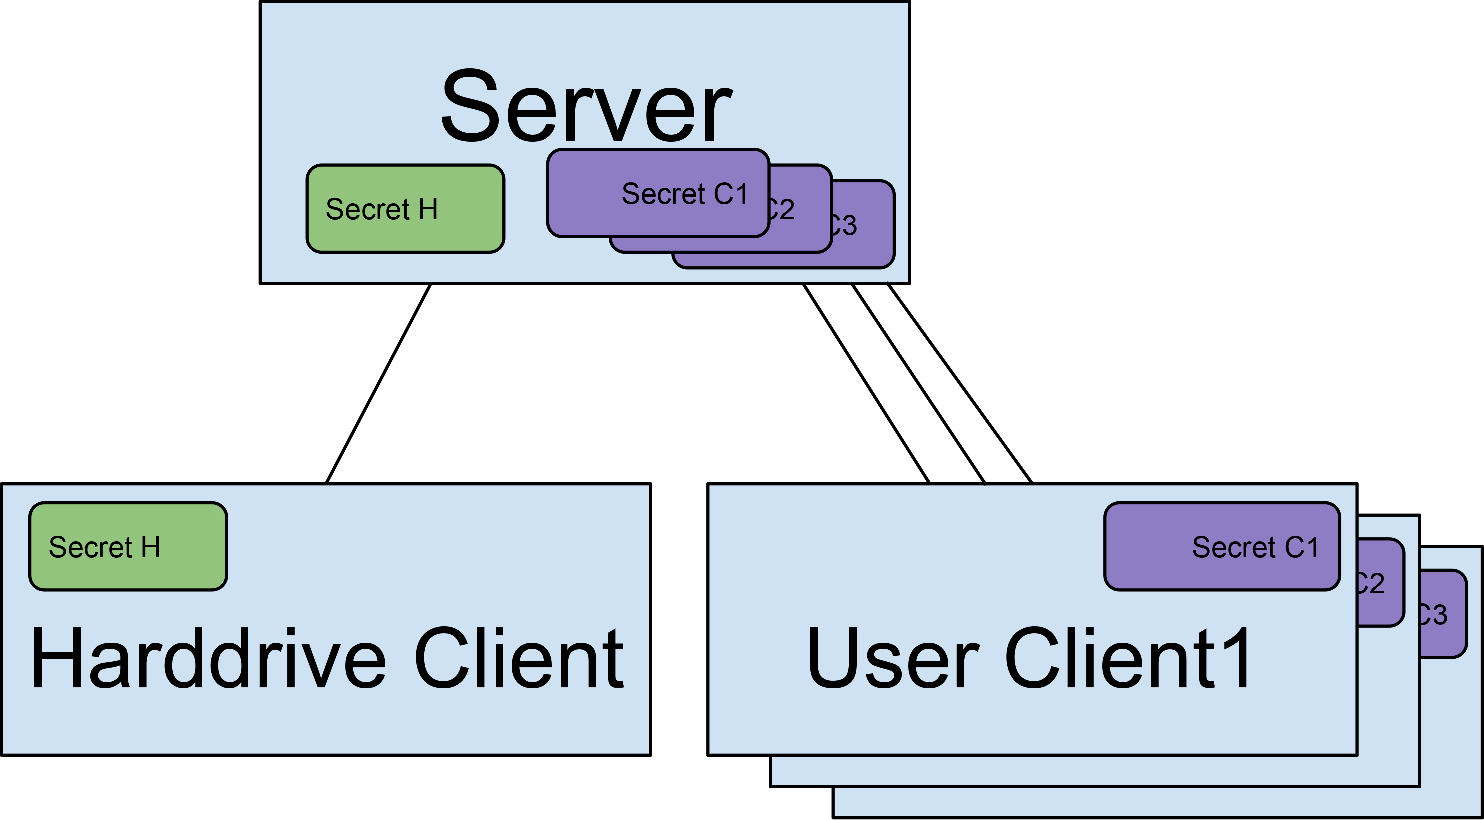
\includegraphics[width=0.7\linewidth]{images/BasicSystem.pdf}}
\caption{System concept. Important to note is that all secrets are stored in encrypted form. Secret in the User Client are stored inside the Yubikey. }\label{fig:basicSystemFigure}
\end{figure}
\begin{figure}[h]
\centerline{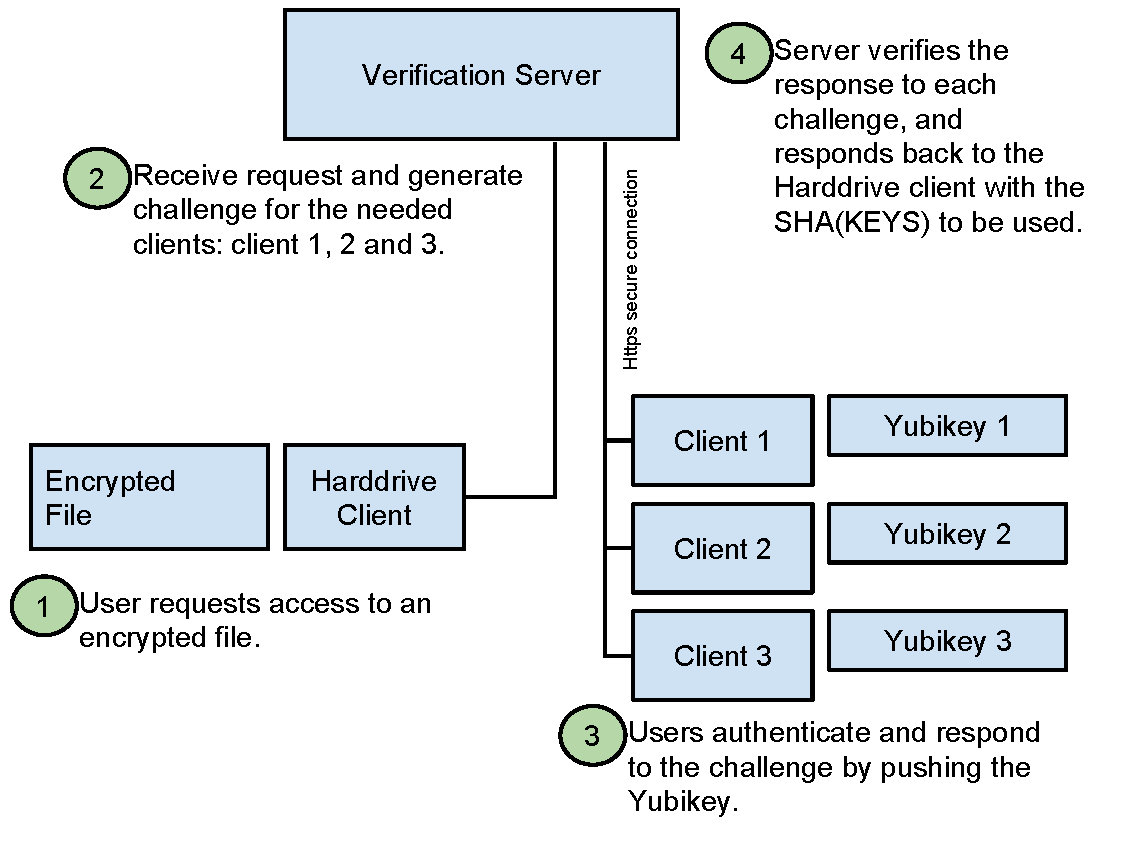
\includegraphics[width=1\linewidth]{images/SystemSteps.pdf}}
\caption{System components and interaction. 4 major steps to grant access.}\label{fig:systemfigure}
\end{figure}

Figure \ref{fig:systemfigure} describes the steps involved with decrypting a file, with a quorum of three clients. Essential to this procedure is that at no point is the actual file key sent ower the network. Only in encrypted form with sequence numbers adding entropy. This is achieved by HMAC-SHA1 encryption of the exchanged data, with the shared secrets.

To give a full overview of what needs to be stored in the indivual parts of the system, figure \ref{fig:detailedsystemfigure} shows a configuration with three user clients.

\begin{figure}[h]
\centerline{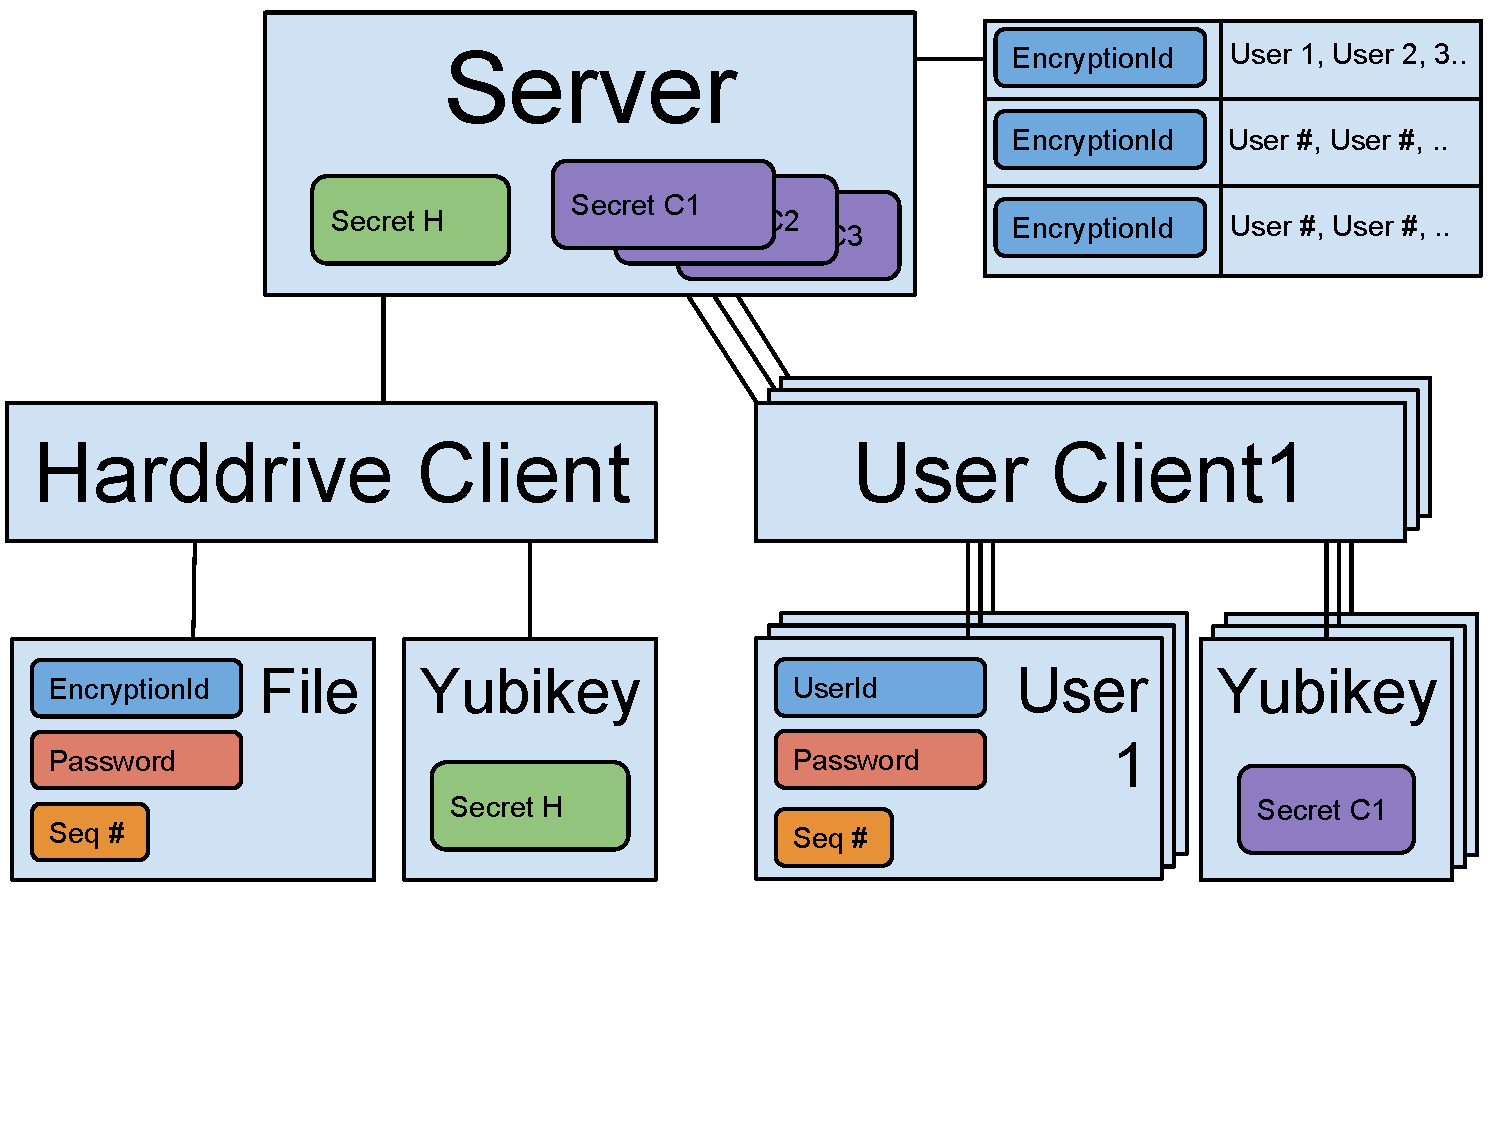
\includegraphics[width=1\linewidth]{images/DetailedSystem.pdf}}
\caption{System with needed variables}\label{fig:detailedsystemfigure}
\end{figure}

\subsection{Multifactor authorization}

Yubikey is a marketed USB dongle used for various Multifactor authentication purposes. It can be set up in different modes, for One Time Password (OTP) based on a series of variables, including sequence numbers. In this work we used the Challenge-Response mode, where the Yubikey is configured with a shared Secret Key among the server and the key itself. The Secret Key is SHA-1 cryptographic hash function. 

Yubikey furthermore provides a simple procedure for the user: only a physical touch on the device is necessary to allow the device to respond to the presented challenge. This is used to ensure that the response is originating from an actual person.

Furthermore, this hardware allows for a secure distribution of shared secrets, as yubikeys can be handed out or shipped to users pre-programmed. Thereby not having to send any shared secrets over the wire.

\begin{figure}[h]
\centerline{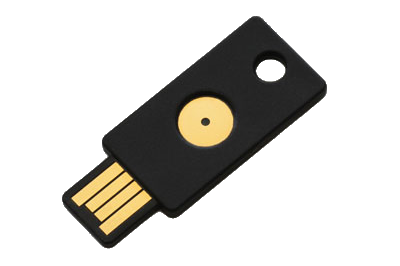
\includegraphics[width=0.3\linewidth]{images/YubiKey_Standard.png}}
\caption{Yubikey capable of performing HMAC-SHA1 encryption with pre-programmed secret.}\label{yubikey}
\end{figure}

\section{Previous work}
We based our model on a proposed hard drive encryption mechanism published on the Yubikey website\cite{YubikeyEncryption}. In their proposed configuration the Yubikey is programmed with a secret key after which it is able to perform HMAC-SHA1 encryption. The device is said to be operating in Challenge-Response mode since you can send it a challenge and it will respond with the HMAC-SHA1 encryption of the challenge with the secret key. This is depicted in figure~\ref{fig:challengeResponse}.


\begin{figure}[h]
\centerline{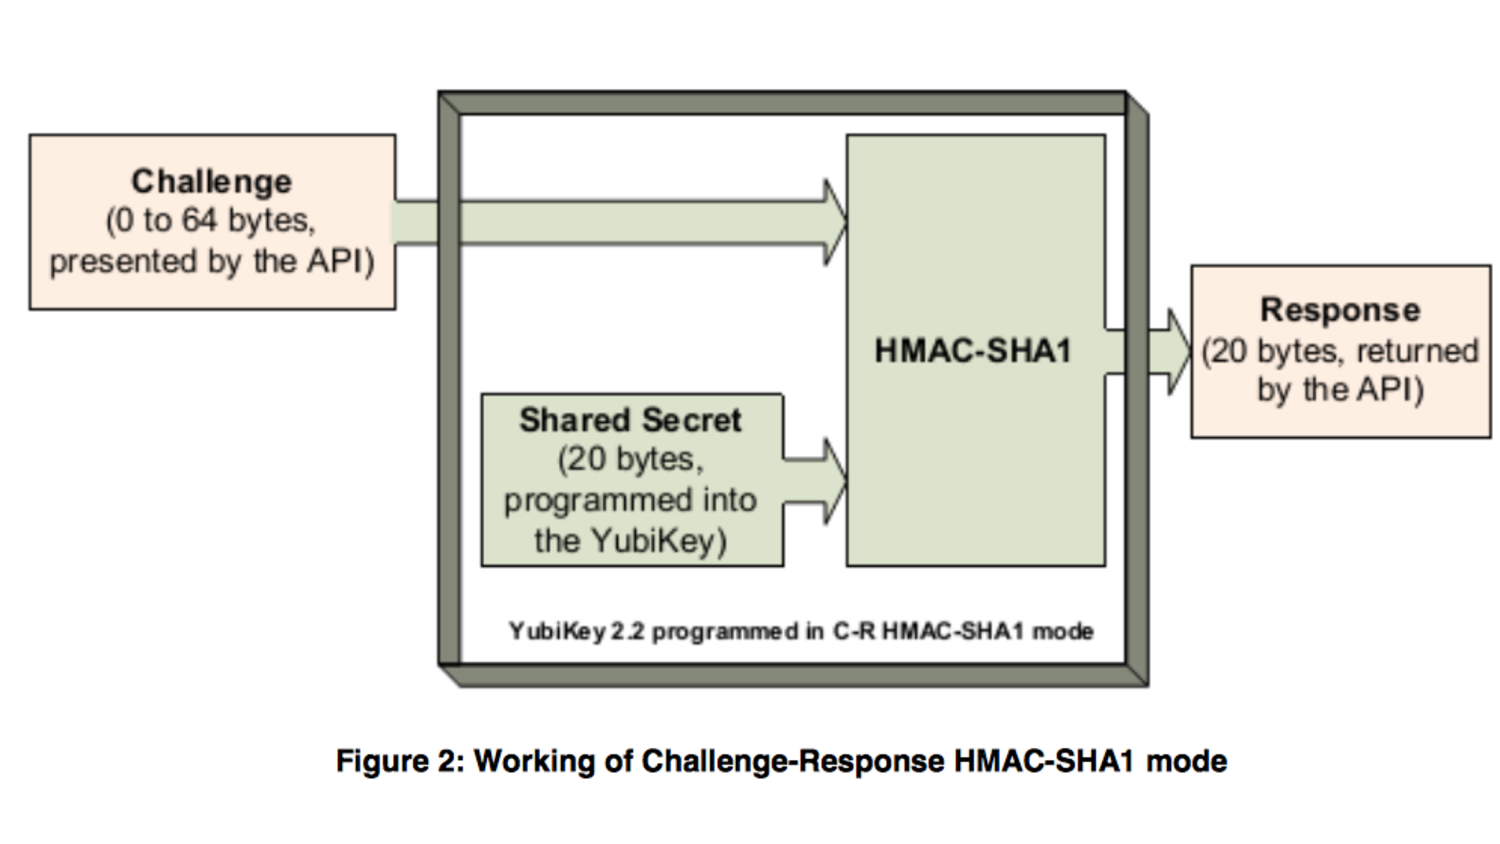
\includegraphics[width=0.7\linewidth]{ChallengeResponseFigure.pdf}}
\caption{Challenge-Response mode of Yubikey.}\label{fig:challengeResponse}
\end{figure}

Figure 2 shows how this mode is used for encrypting a local hard drive. The hard drive is encrypted with a Drive Encryption Key (DEK) which is stored in a table along with the secret. Both are encrypted using AES. The key used for the encryption is shown in Figure 2. Once the user enters his password a challenge is generated. The challenge consists of the password itself and a sequence number (Seq) that is also stored in the table. This challenge is sent to the Yubikey, whose response allows us to decrypt the DEK and the secret. The hard drive can now be decrypted. After decryption the DEK is re-encrypted with a new sequence number and the secret.

\begin{figure}[h]
\centerline{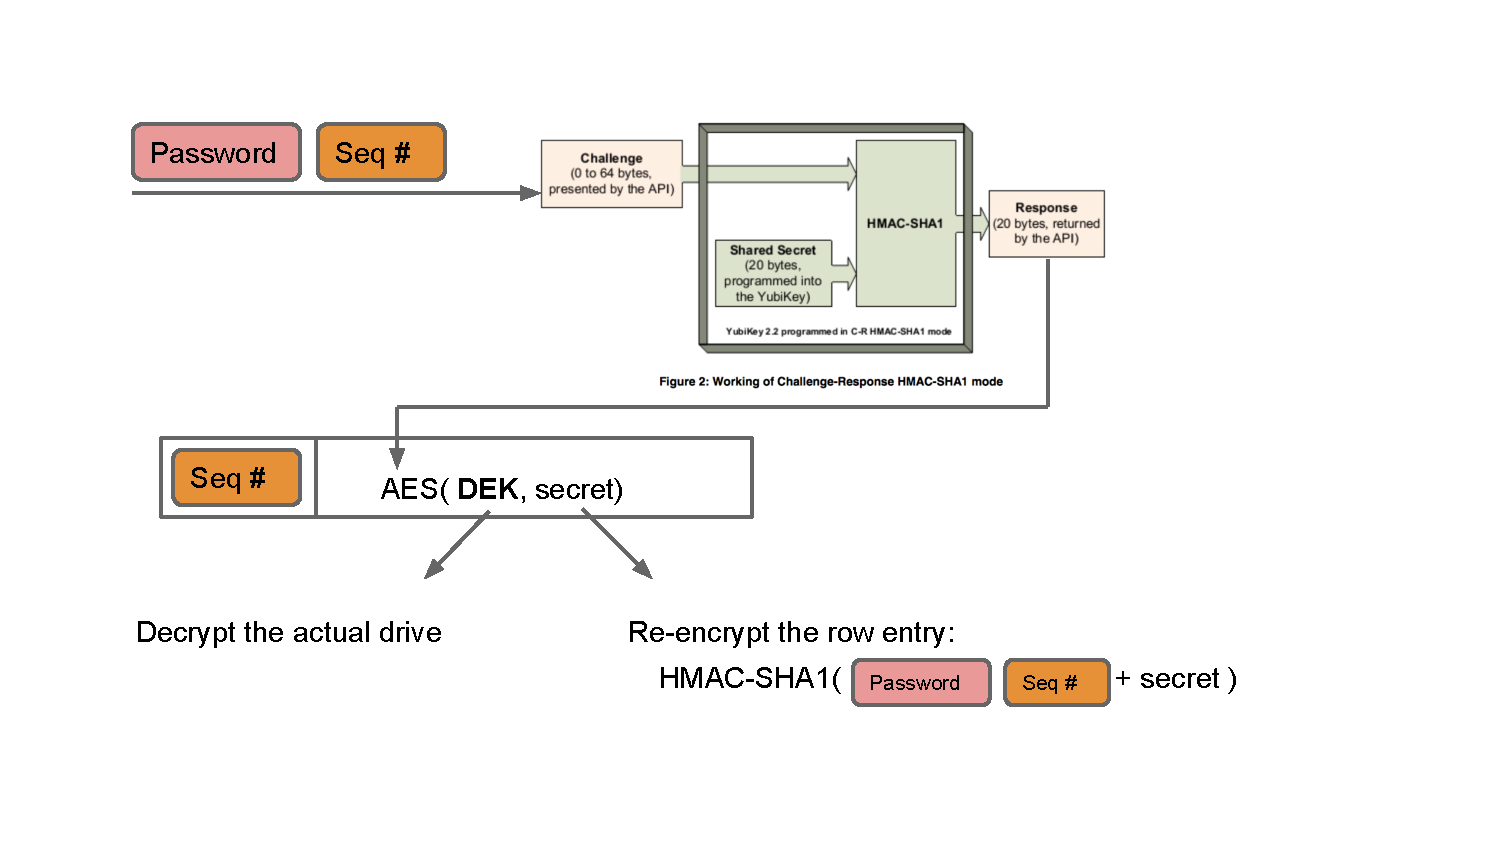
\includegraphics[width=1\linewidth]{HardDriveEncryptionFigure.pdf}}
\caption{Local hard drive encryption configuration.}\label{fig:harddriveEncryption}
\end{figure}

%------------------------------------------------


\section{Encryption scheme}

This sections presents the encryption scheme used, to ensure that decryption of the file is only possible when responses from all participants and their Yubikey challenges are retrieved. 

\subsection{Setup Of Quorum}

When a user is added to the server, he is given a secret key by the server that is written into the Yubikey. 

The hard drive host (the client program that is in charge of decrypting the drive) generates a Drive Encryption Key (DEK) to encrypt the hard drive with. Once encrypted, it sends a request to the server to set up a quorum of users with which it wants to share the encryption. The server responds with an encryptionId and a secret cryptographic hash \( SHA(\sum key) \). This hash, along with the DEK are AES-encrypted and stored on the hard drive host. The key used for the encryption is calculated as follows:
\begin{equation}
	encryptionKey = HMACSHA1( challenge, SHA(\sum key))
\end{equation}
\begin{equation}
	challenge = SHA(encryptionId + seq + password)
\end{equation}
The seq is a sequence number that is used to provide entropy to the challenge, it is also stored on the host. The password is necessary to generate the challenge in the future, and is global to this hard drive, not specific to any particular user in the quorum. After this encryption the hard drive host no longer has access to the DEK or the \( SHA(\sum key) \).

During the setup phase the server generates a key for each user in the quorum such that it is unique for the user-encryptionId pair. These keys are used to compute the \( SHA(\sum key) \) cryptographic hash used above.

\section{Key Generation and Storage}

When the server generates a unique key for the user-encryptionId pair, it immediately AES-encrypts it along with the users's secret. It uses the following encryptionKey for the encryption:

\begin{equation}
	encryptionKey = HMACSHA1( challenge, secret)
\end{equation}
\begin{equation}
	challenge = SHA(encryptionId + userId + seq)
\end{equation}

Note that after this encryption, the unique key and the user's secret are encrypted away. 

\section{Decryption Process}
When the hard drive host wants to decrypt the hard drive, it sends a request to the server with the corresponding encryptionId. Along with the request, it also sends a challenge:

\begin{equation}
challenge = SHA(encryptionId + seq + password)
\end{equation}

Note that in order to decrypt the DEK the server needs to obtain: \( HMACSHA1( challenge, SHA(\sum key)) \). Upon receiving the request the server needs to gain access to the keys of all the users that are part of the quorum so that it can generate \( SHA(\sum key) \). In order to do so it sends each user a challenge:

\begin{equation}
	challenge = SHA(encryptionId + userId + seq)
\end{equation}

The user responds with \( HMACSHA1( challenge, secret) \) using their Yubikey. This response can be used to decrypt the key that belongs to the encryptionId-user pair. Once all the users have responded we now can calculate \( SHA(\sum key) \). At this point we no longer need the individual keys, and they can be re-encrypted with incremented sequence numbers. Now we return  \( HMACSHA1( challenge, SHA(\sum key)) \) to the hard drive host. 

The hard drive host now decrypts the DEK and the hard drive. Immediately it re-encrypts the DEK with an incremented sequence number.

\section{Security Evaluation}
We evaluate the security of the proposed system by considering various attack vectors. We leave the evaluation of specific encryption and hashing mechanisms to other work, and assume them to be computationally unreasonably hard to break. We also do not evaluate the security implications of specifically using the Yubikey product, Yubico provides a detailed evaluation on their website \cite{YubikeySecurity}. 

\subsection{Server Attacks}
In designing the server side component we took deliberate care not to expose enough information to compromise the security of the hard drive at any point in the future. The database on the server stores the following items:
\begin{itemize}
	\item Yubikey secret of each user (AES encrypted)
	\item Key that corresponds to the user's share of an encrypted hard drive (AES encrypted)
	\item Mapping of hard drive to users who belong to the encryption
	\item Sequence number used for obfuscation
\end{itemize}
In order to decrypt the secret or the key, the attacker would need to gain access to the user's secret in order to be able to generate the decryption key via a HMAC-SHA1 algorithm. While the server does not provide any additional protection if the user secret has been compromised, it does not make matters any worse. Furthermore all users of a particular hard drive would need to be compromised in this way for a successful decryption. This is analogous to finding out everyone's password\todo{dont you mean secret? As that is stored on the yubikey. The password the user just knows, so that it is actually multifactor..}, which is stored on their YubiKey device.

\todo{Should we discuss the attack where the attacker takes over the server, and sends out requests to users to gain access to files ? .. it is maybe a bit sought for, as he would also need to compromise the harddrive client in order to gain access to the actual file..}

\subsection{Network Attacks}
All communications are assumed to be SSL encrypted in a production environment to provide the first layer of security. With that in mind, let us consider what data is sent over the network during the decryption process.

\subsubsection{Between Client and Server}
When the client initiates a decryption, it sends over an \textbf{encryptionId} and a challenge. The encryptionId which is used to identify the hard drive and associated users. The challenge is a SHA hash of the encryptionId, a sequence number (seq) and an optional password. Finally the server will answer with a response.
\begin{itemize}
	\item encryptionId
	\item challenge \( \Rightarrow  SHA(encryptionId, seq, password) \)
	\item response \( \Rightarrow HMACSHA1(challenge, SHA( \sum Keys)) \)
\end{itemize}
The challenge and the response leak no data, nor are they useful in a future decryption attempt since the sequence number will have changed. The encryptionId is in itself not of much use, however if somebody had also access to the server database, they would be able to find out which users are participating in a decryption. Even then, they would still need to attain the secret's of all the users to be able to decrypt their keys.

\subsubsection{Between Server and Users}
Between the server and users, only challenge and response are exchanged over the wire. These change every request due to per-user sequence numbers thus intercepting these would not lead to future vulnerabilities.

\subsection{Hard Drive host attacks}
If the hard drive host is compromised, it could issue a decryption request to the server. For this attack vector to work, all the users would need to respond to the challenges. Without the server's approval the attacker would not gain access to the DEK. If the hard drive host is compromised during a legitimate decryption, it could also obtain the DEK by reading it from the program's memory, we consider such an attack very difficult to mount.

\subsection{Client User Attacks}
A compromised client could potentially respond to challenges programatically. The Yubikey provides a setting, where a button press is required in order to respond to a challenge, this precaution will prevent automated responses.

\subsection{Key Entropy}
In our prototype we naively implemented \( SHA(\sum key) \) by simply summing the keys together and taking the SHA hash. This potentially reduces the entropy of the key and is a potential attack vector. Future work in cleverly combining the user keys may alleviate this concern.

%------------------------------------------------

\section{Conclusion}

We have presented a system for distributing file access to a quorum of users. Users request to encrypt/decrypt files by sending a challenge to a server. The server distributes new challenges to the quorum of users that correspond to the encryption. Only after all participants of the quorum have responded, the server is able to generate an appropriate response to the hard drive client that can be used to decrypt the DEK (Drive Encryption Key) and ultimately the file.

Various attack vectors on this system have been identified, with the most vulnerable points being whenever the actual sum of all quorum keys are held in memory. This happens for a short while on both the server and the hard drive client. In both cases, this value is quickly re-encrypted again with an incremented sequence number. Also, during the initialization process, the shared secrets are temporarily vulnerable, which can be alleviated by shipping these in pre-programmed dedicated hardware devices, for instance Yubikeys.

%----------------------------------------------------------------------------------------
%	ACKNOWLEDGEMENTS
%----------------------------------------------------------------------------------------

%\pagebreak

%\begin{acknowledgments}
%This work was supported by..
%\end{acknowledgments}

%----------------------------------------------------------------------------------------
%	BIBLIOGRAPHY
%----------------------------------------------------------------------------------------

\begin{thebibliography}{10}


\bibitem{UserLock}
http://www.isdecisions.com/lp/userlock/userlock-windows-network-security.htm?gclid=CMfPl-rqisQCFciBfgodhxwAmQ

\bibitem{CLAcha1}
http://software.dell.com/products/identity-manager-data-governance/

\bibitem{YubikeyEncryption}
https://www.yubico.com/applications/disk-encryption/full-disk-encryption/

\bibitem{YubikeySecurity}
https://www.yubico.com/wp-content/uploads/2012/10/Security-Evaluation-v2.0.1.pdf

\end{thebibliography}

%----------------------------------------------------------------------------------------

\end{article}

\end{document}